
\section{Introduction}

Classes scheduling is a \emph{constraints satisfaction problem} (CSP).
and all scheduling problems share a common constraint: schedule consistency ---
one cannot participate in several events at the same time. For the classes case,
the participants are:
\begin{enumerate*}
  \item \emph{groups} of students,
  \item teachers or \emph{professors},
  \item \emph{classrooms}.
\end{enumerate*}
The first two are represented by real people and the rooms are represented by
the institution.

Problem \emph{constraints} can be divided into:
\begin{enumerate}
  \item \underline{Class constraints}: a class should be a productive event, so
    a professor should be able to \emph{teach} the class, the classroom should
    have the \emph{capacity} to hold all the students and be properly \emph{equipped},
    and the group should be \emph{inscribed} to class subject
    (further called \emph{discipline}).
  \item \underline{Time constraints}: no participant can have two classes
    at the same time (or intersecting in time), as mentioned before.
  \item \underline{Strong restrictions}: the restrictions, put on a participant, that
    \emph{must} be respected. May include working hours, fixed lunch recess time,
    and any other institution or person specific \emph{obligations}.
  \item \underline{Weak restrictions}: the restrictions, that \emph{should} be respected,
    but are not critical to the solution. Compliance with theese restrictions
    raises \emph{solution quality}, but it is assumed that the all of them
    cannot be fully met for all the participants --- they are intended to
    represent personal \emph{preferences}.
\end{enumerate}

The goal is finding a solution --- schedule, satisfying all the constraints.
University schedule is composed of \emph{individual schedules} for every
participant. An individual schedules may be seen as a day-time table with
classes in the cells. Therefore the complete schedule can be represented as a
3-dimentional table, as shown in figure \ref{fig:ScheduleSpace}.
\bigskip

\begin{figure}
  \label{fig:ScheduleSpace}
  
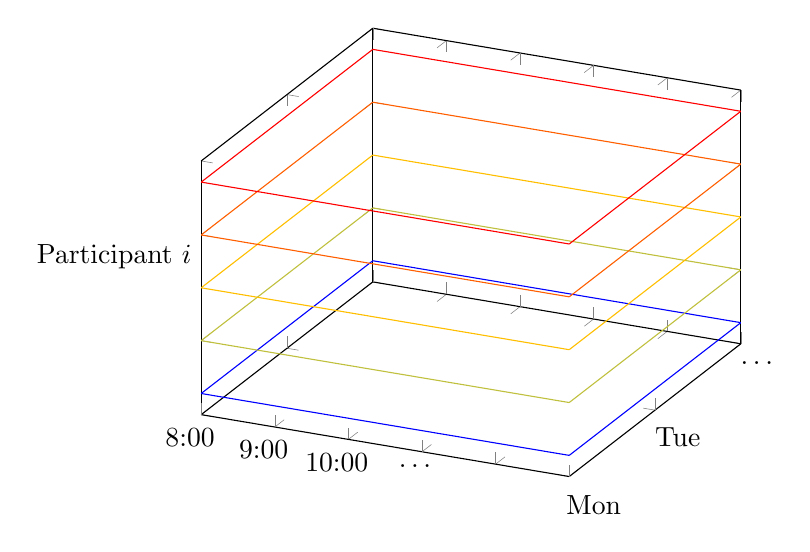
\begin{tikzpicture}

\begin{axis}[
  xlabel=, % Time,
  xticklabels={, 8:00, 9:00, 10:00, $\dots$},
  ylabel=, %Day,
  yticklabels={, Mon, Tue, $\dots$},
  zlabel=, %Participant,
  zticklabels = {, , ,Participant $i$}
  ]

  \foreach \i in {1,...,5}
     \addplot3[surf] coordinates { (0,0,\i) (1,0,\i) (1,1,\i) (0,1,\i) (0,0,\i)  };

  % \addplot3[surf] coordinates { (0,0,0) (1,0,0) (1,1,0) (0,1,0) (0,0,0)  };
  % \addplot3[surf] coordinates { (0,0,1) (1,0,1) (1,1,1) (0,1,1) (0,0,1)  };

\end{axis}


\end{tikzpicture}

  \caption{University schedule is a 3-dimentional table. Horizontal rectangles
           represent invividual schedules for the corresponding participants.
          }
\end{figure}


Scheduling problems are \emph{n-p complete} \cite{ULLMAN1975384}
and therefore the optimal solution can be found within finite (polynomial) time.
But being finite, doesn't make the required time acceptable.
To ensure solution perfection, one must consider \emph{every possible} classes
configuration.

For example, six working days in a week and twelve time slots every day
(every hour from 8:00 to 20:00), would yield $6 \times 12 = 72$ options
to place each class.
Given that each group needs five diferent disciplines to be asssigned,
there would be  $\multibinom{72}{5} = 18474840$ possible classes assignment for
each group (without considering professors and classrooms).
Thus, the time, required to find the \emph{optimal solution}, might exceed any
reasonable limits, if the university is big.

This problem is a typical one for the CSPs, and many researchers have
been looking for means of solving such problems within reasonable time.
During the last years different algorithms and techniques where developed,
such as
\emph{dynamic constraint satisfaction based on extension particle swarm
      optimization algorithm} \cite{CSPswarm},
\emph{dynamic state bounding} \cite{CSPdynStateBound},
\emph{conflict-vector detection} \cite{CSPtimetable},
\emph{neural networks} \cite{CSPneuro},
\emph{ant colony optimization} \cite{CSPcunningACO, CSPlimmemACO},
\emph{selective hyper-heuristics} \cite{CSPhypHeur}
and \emph{agents} \cite{CSPagent2013, CSPagent2014, DCSPagent1998}.


The \emph{agent negotiation} approach is usually used for solving distributed
CSPs (DCSPs) \cite{DCSPagent1998, DCSP2013, CSPagent2014}.
In this case the constrains are \emph{distributed} among the agents instead of
being gathered in one place.

\red{Such constraints distribution is useful for the \emph{classes scheduling} problem
, because it permits to distribute not only the constraints, but also the solution. }
Each agent would be expected to \emph{negotiate} a suitable solution for its
``master'', without concerning itself with the schedules of the others.
Tthe combined solution can be obtained as soon as all the participants agree on
their timetables.
